\documentclass{beamer}
\usepackage{beamerthemesplit}
\usepackage{wrapfig}
\usetheme{SPbGU}
\usepackage{pdfpages}
\usepackage{amsmath}
\usepackage{mathtools}
\usepackage{cmap} 
\usepackage[T2A]{fontenc} 
\usepackage[utf8]{inputenc}
\usepackage[english,russian]{babel}
\usepackage{indentfirst}
\usepackage{amsmath}
\usepackage{tikz}
\usepackage{multirow}
\usepackage[noend]{algpseudocode}
\usepackage{algorithm}
\usepackage{algorithmicx}
\usepackage{ stmaryrd }
\usepackage{fancyvrb}
\usepackage{qtree}
\usepackage{verbatim}
\newtheorem{rutheorem}{Теорема}
\newtheorem{ruproof}{Доказательство}
\newtheorem{rudefinition}{Определение}
\newtheorem{rulemma}{Лемма}
\beamertemplatenavigationsymbolsempty

\setbeamertemplate{itemize item}[circle]
\setbeamertemplate{enumerate item}[circle]
\newcommand{\derives}[1][*]{\xRightarrow[]{#1}}

\newenvironment{myauto}[1][3]
{
  \begin{center}
    \begin{tikzpicture}[> = stealth,node distance=#1cm, on grid, very thick]
}
{
    \end{tikzpicture}
  \end{center}
}

\def\To{\derives[]}
\def\iff{\Leftrightarrow}

\usetikzlibrary{shapes,arrows}
\usetikzlibrary{positioning,automata}
\tikzset{
  every state/.style={minimum size=0.2cm},
  initial text={}
}

\title[]{Теория автоматов и формальных языков}
\subtitle[]{Регулярные языки}
\institute[]{
Санкт-Петербургский государственный электротехнический университет <<ЛЭТИ>>\\
}

\author[]{Екатерина Вербицкая}

\date{26 сентября 2019}

\definecolor{orange}{RGB}{179,36,31}

\begin{document}
{
  \begin{frame}
    \titlepage
  \end{frame}
}


\begin{frame}[fragile]
  \transwipe[direction=90]
  \frametitle{В предыдущей серии}
  \textbf{Конечный автомат} --- $\langle Q, \Sigma, \delta, q_0, F \rangle$

  \begin{itemize}
    \item $Q \neq \varnothing$ --- конечное множество состояний
    \item $\Sigma$ --- Конечный входной алфавит
    \item $\delta$ --- функция переходов
    \begin{itemize}
      \item Детерминированный КА: отображение типа $Q \times \Sigma \to Q$
      \item Недетерминированный КА: отображение типа $Q \times \Sigma \to 2^Q$
    \end{itemize}
    \item $q_0 \in Q$ --- начальное состояние
    \item $F \subseteq Q$ --- множество конечных состояний
  \end{itemize}
\end{frame}

\begin{frame}[fragile]
  \transwipe[direction=90]
  \frametitle{В предыдущей серии: ДКА}
    \begin{myauto}
      \node[state,initial]   (q_01)                      {A};
      \node[state]           (q_2)  [right=of q_01]      {B};
      \node[state,accepting] (q_3)  [right=of q_2]       {C};
      \node[state]           (q_4)  [above right=of q_3] {D};
      \node[state]           (q_56) [below right=of q_3] {E};
  
      \path[->] (q_01) edge [loop above]    node [above] {$1$} ()
                       edge [bend left=15]  node [above] {$0$} (q_2)
                (q_2)  edge                 node [below] {$1$} (q_3)
                       edge [bend left=15]  node [below] {$0$} (q_01)
                (q_3)  edge [bend left=15]  node [above] {$1$} (q_56)
                       edge                 node [above] {$0$} (q_4)
                (q_4)  edge [loop above]    node [left]  {$1$} ()
                       edge [loop right]    node [right] {$0$} ()
                (q_56) edge [bend left=15]  node [below] {$1$} (q_3)
                       edge                 node [right] {$0$} (q_4);
    \end{myauto} 
\end{frame}

\begin{frame}[fragile]
  \transwipe[direction=90]
  \frametitle{В предыдущей серии: распознавание слова ДКА}
  \begin{myauto}
    \node[state,initial]   (q_01)                      {A};
    \node[state]           (q_2)  [right=of q_01]      {B};
    \node[state,accepting] (q_3)  [right=of q_2]       {C};
    \node[state,thin]      (q_4)  [above right=of q_3] {D};
    \node[state,thin]      (q_56) [below right=of q_3] {E};

    \path[->] (q_01) edge [loop above, thin]    node [above] {$1$} ()
                     edge [bend left=15]        node [above] {$0$} (q_2)
              (q_2)  edge                       node [below] {$1$} (q_3)
                     edge [bend left=15, thin]  node [below] {$0$} (q_01)
              (q_3)  edge [bend left=15, thin]  node [above] {$1$} (q_56)
                     edge [thin]                node [above] {$0$} (q_4)
              (q_4)  edge [loop above, thin]    node [left]  {$1$} ()
                     edge [loop right, thin]    node [right] {$0$} ()
              (q_56) edge [bend left=15, thin]  node [below] {$1$} (q_3)
                     edge [thin]                node [right] {$0$} (q_4);
  \end{myauto} 
\end{frame}

\begin{frame}[fragile]
  \transwipe[direction=90]
  \frametitle{В предыдущей серии: распознание слова ДКА}
  \begin{myauto}
    \node[state,initial]   (q_01)                      {A};
    \node[state]           (q_2)  [right=of q_01]      {B};
    \node[state,accepting] (q_3)  [right=of q_2]       {C};
    \node[state,thin]      (q_4)  [above right=of q_3] {D};
    \node[state,thin]      (q_56) [below right=of q_3] {E};

    \path[->] (q_01) edge [loop above]          node [above] {$1$} ()
                     edge [bend left=15]        node [above] {$0$} (q_2)
              (q_2)  edge                       node [below] {$1$} (q_3)
                     edge [bend left=15, thin]  node [below] {$0$} (q_01)
              (q_3)  edge [bend left=15, thin]  node [above] {$1$} (q_56)
                     edge [thin]                node [above] {$0$} (q_4)
              (q_4)  edge [loop above, thin]    node [left]  {$1$} ()
                     edge [loop right, thin]    node [right] {$0$} ()
              (q_56) edge [bend left=15, thin]  node [below] {$1$} (q_3)
                     edge [thin]                node [right] {$0$} (q_4);
  \end{myauto} 
\end{frame}

\begin{frame}[fragile]
  \transwipe[direction=90]
  \frametitle{В предыдущей серии: распознание слова ДКА}
  \begin{myauto}
    \node[state,initial]   (q_01)                      {A};
    \node[state]           (q_2)  [right=of q_01]      {B};
    \node[state,accepting] (q_3)  [right=of q_2]       {C};
    \node[state,thin]      (q_4)  [above right=of q_3] {D};
    \node[state]           (q_56) [below right=of q_3] {E};

    \path[->] (q_01) edge [loop above]          node [above] {$1$} ()
                     edge [bend left=15]        node [above] {$0$} (q_2)
              (q_2)  edge                       node [below] {$1$} (q_3)
                     edge [bend left=15, thin]  node [below] {$0$} (q_01)
              (q_3)  edge [bend left=15]        node [above] {$1$} (q_56)
                     edge [thin]                node [above] {$0$} (q_4)
              (q_4)  edge [loop above, thin]    node [left]  {$1$} ()
                     edge [loop right, thin]    node [right] {$0$} ()
              (q_56) edge [bend left=15]        node [below] {$1$} (q_3)
                     edge [thin]                node [right] {$0$} (q_4);
  \end{myauto}
  
  
  \begin{center}
    Слово распознается за $O(n)$
  \end{center}
\end{frame}

\begin{frame}[fragile]
  \transwipe[direction=90]
  \frametitle{В предыдущей серии: распознание слова НКА}
  \begin{myauto}[2.5]
    \node[state,accepting] (q_2)                 {C};
    \node[state,initial]   (q_0)  [left=of q_2]  {A};
    \node[state,accepting] (q_1)  [above=of q_2] {B};
    \node[state]           (q_3)  [below=of q_2] {D};
    \node[state,accepting] (q_4)  [right=of q_1] {E};
    \node[state]           (q_5)  [right=of q_2] {F};

    \path[->] (q_0) edge                node [above] {$a$} (q_1)
                    edge                node [above] {$a$} (q_2)
                    edge                node [above] {$a$} (q_3)
              (q_1) edge                node [above] {$b$} (q_4)
              (q_3) edge [bend left=15] node [above] {$b$} (q_5)
              (q_4) edge [loop below]   node [below] {$b$} ()
              (q_5) edge [bend left=15] node [below] {$a$} (q_3)
              (q_5) edge                node [above] {$a$} (q_2)
              ;
  \end{myauto} 

  
  \begin{center}
    Слово распознается за $O(|\omega| \sum\limits_{t \in Q} \sum\limits_{c \in \Sigma} |\delta(t, c)|)$
  \end{center}
\end{frame}

\begin{frame}[fragile]
  \transwipe[direction=90]
  \frametitle{В предыдущей серии: детерминизация}
  \begin{myauto}
    \node[state,accepting] (q_2)                 {E};
    \node[state,initial]   (q_0)  [left=of q_2]  {A};
    \node[state,accepting] (q_1)  [above=of q_0] {BCD};
    \node[state,accepting] (q_3)  [above=of q_2] {EF};
    \node[state]           (q_4)  [right=of q_2] {F};
    \node[state,accepting] (q_5)  [above=of q_4] {CD};

    \path[->] (q_0) edge                node [left]  {$a$} (q_1)
              (q_1) edge                node [above] {$b$} (q_3)
              (q_2) edge [loop left]    node [left]  {$b$} ()
              (q_3) edge                node [left]  {$b$} (q_2)
                    edge                node [above] {$a$} (q_5)
              (q_4) edge [bend left=15] node [left]  {$a$} (q_5)
              (q_5) edge [bend left=15] node [right] {$b$} (q_4)
              ;
  \end{myauto}

\end{frame}

\begin{frame}[fragile]
  \transwipe[direction=90]
  \frametitle{В предыдущей серии: минимизация}
  \begin{center}
    \resizebox{!}{0.4\textheight}{
      \begin{tikzpicture}[> = stealth,node distance=3cm, on grid, very thick]
        \node[state]           (q_2)                      {C};
        \node[state,initial]   (q_0) [above left=of q_2]  {A};
        \node[state]           (q_1) [below left=of q_2]  {B};
        \node[state]           (q_3) [right=of q_2]       {D};
        \node[state]           (q_4) [above right=of q_3] {E};
        \node[state,accepting] (q_5) [below right=of q_3] {F};
        \node[state,accepting] (q_6) [above right=of q_5] {G};
    
        \path[->] (q_0) edge [bend left=15]  node [right] {$1$} (q_1)
                        edge                 node [above] {$0$} (q_2)
                  (q_1) edge [bend left=15]  node [left]  {$1$} (q_0)
                        edge                 node [below] {$0$} (q_2)
                  (q_2) edge [bend right=15] node [below] {$1$} (q_3)
                        edge [bend left=15]  node [above] {$0$} (q_3)
                  (q_3) edge                 node [below] {$1$} (q_5)
                        edge                 node [above] {$0$} (q_4)
                  (q_4) edge                 node [above] {$1$} (q_6)
                        edge                 node [right] {$0$} (q_5)
                  (q_5) edge [loop below]    node         {$1$} ()
                        edge [loop left]     node         {$0$} ()
                  (q_6) edge                 node [below] {$1$} (q_5)
                        edge [loop right]    node         {$0$} ();
      \end{tikzpicture}
    }
  \end{center}
  

  \begin{center}
    \resizebox{!}{0.4\textheight}{
      \begin{tikzpicture}[> = stealth,node distance=3cm, on grid, very thick]
        \node[state,initial]   (q_01)                     {AB};
        \node[state]           (q_2)  [right=of q_01]      {C};
        \node[state]           (q_3)  [right=of q_2]       {D};
        \node[state]           (q_4)  [above right=of q_3] {E};
        \node[state,accepting] (q_56) [below right=of q_3] {FG};
    
        \path[->] (q_01) edge [loop above]    node [above] {$1$} ()
                         edge                 node [above] {$0$} (q_2)
                  (q_2)  edge [bend right=15] node [below] {$1$} (q_3)
                         edge [bend left=15]  node [above] {$0$} (q_3)
                  (q_3)  edge                 node [below] {$1$} (q_56)
                         edge                 node [above] {$0$} (q_4)
                  (q_4)  edge [bend right=15] node [left]  {$1$} (q_56)
                         edge [bend left=15]  node [right] {$0$} (q_56)
                  (q_56) edge [loop below]    node         {$1$} ()
                         edge [loop left]     node         {$0$} ();
      \end{tikzpicture}
    }
  \end{center}

\end{frame}

\begin{frame}[fragile]
  \transwipe[direction=90]
  \frametitle{Произведение автоматов}
   $A_1 = \langle \Sigma_1, Q_1, q_{1_0}, \delta_1, F_1 \rangle$ и $A_2 = \langle \Sigma_2, Q_2, q_{2_0}, \delta_2, F_2 \rangle$ --- КА
  
   \vfill 

  \textbf{Произведением} автоматов назовем $A = \langle \Sigma, Q, q_0, \delta, F \rangle$, где

  \vfill

  \begin{itemize}
    \item $\Sigma = \Sigma_1 \cup \Sigma_2$
    \item $Q = Q_1 \times Q_2$
    \item $q_0 = (q_{1_0}, q_{2_0})$
    \item $F \subseteq Q$
    \begin{itemize}
      \item $F = F_1 \times F_2$ --- распознает \textbf{пересечение} языков
      \item $F = (F_1 \times Q_2) \cup (Q_1 \times F_2)$ --- распознает \textbf{объединение} языков
      \item $F = F_1 \times (Q_2 \setminus F_2)$ --- распознает \textbf{разность} языков
    \end{itemize}
    \item $\delta((q_1, q_2), c) = (\delta_1(q_1, c), \delta_2(q_2, c))$
  \end{itemize}
  
  \vfill 

  Интуиция: ищем пути в двух автоматах одновременно
\end{frame}


\begin{frame}[fragile]
  \transwipe[direction=90]
  \frametitle{Произведение автоматов: пример}
  \begin{columns}
    \begin{column}{0.4\textwidth}
      \begin{myauto}[2]
        \node[state,initial]   (q_0)                {A};
        \node[state,accepting] (q_1) [right of=q_0] {B}; 
    
        \path[->] (q_0) edge [loop above] node [above] {$0$}    ()
                        edge              node [above] {$1$}    (q_1)
                  (q_1) edge [loop above] node [above] {$0, 1$} ();
      \end{myauto}    
    \end{column}

    \begin{column}{0.6\textwidth}
      \begin{myauto}[2]
        \node[state,initial]   (p_0)                {X};
        \node[state]           (p_1) [right of=q_0] {Y}; 
        \node[state,accepting] (p_2) [right of=q_1] {Z};
    
        \path[->] (p_0) edge [loop above] node [above] {$1$}    ()
                        edge              node [above] {$0$}    (p_1)
                  (p_1) edge [loop above] node [above] {$0$}    ()
                        edge              node [above] {$1$}    (p_2)
                  (p_2) edge [loop above] node [above] {$0, 1$} ()
                  ;
      \end{myauto}
    \end{column}
  \end{columns}

  \begin{myauto}[2.3]
    \node[state,initial]   (s_00)                 {A,X}; 
    \node[state]           (s_01) [right of=s_00] {A,Y};
    \node[state,thin]      (s_02) [right of=s_01] {A,Z};
    \node[state]           (s_10) [below of=s_00] {B,X};
    \node[state]           (s_11) [below of=s_01] {B,Y};
    \node[state]           (s_12) [below of=s_02] {B,Z};
    
    \path[->] (s_00) edge                    node [above] {$0$}   (s_01)
                     edge                    node [left]  {$1$}   (s_10)
              (s_01) edge [loop above]       node [above] {$0$}   ()
                     edge                    node [right] {$1$}   (s_12)
              (s_02) edge [loop above, thin] node [above] {$0$}   ()
                     edge [thin]             node [right] {$1$}   (s_12)
              (s_10) edge [loop below]       node [below] {$1$}   ()
                     edge                    node [above] {$0$}   (s_11)
              (s_11) edge [loop below]       node [below] {$0$}   ()
                     edge                    node [above] {$1$}   (s_12)
              (s_12) edge [loop right]       node [right] {$0,1$} (s_12)
              ;
  \end{myauto}
\end{frame}

\begin{frame}[fragile]
  \transwipe[direction=90]
  \frametitle{Пересечение языков}
  \begin{columns}
    \begin{column}{0.4\textwidth}
      \begin{myauto}[2]
        \node[state,initial]   (q_0)                {A};
        \node[state,accepting] (q_1) [right of=q_0] {B}; 
    
        \path[->] (q_0) edge [loop above] node [above] {$0$}    ()
                        edge              node [above] {$1$}    (q_1)
                  (q_1) edge [loop above] node [above] {$0, 1$} ();
      \end{myauto}    
    \end{column}

    \begin{column}{0.6\textwidth}
      \begin{myauto}[2]
        \node[state,initial]   (p_0)                {X};
        \node[state]           (p_1) [right of=q_0] {Y}; 
        \node[state,accepting] (p_2) [right of=q_1] {Z};
    
        \path[->] (p_0) edge [loop above] node [above] {$1$}    ()
                        edge              node [above] {$0$}    (p_1)
                  (p_1) edge [loop above] node [above] {$0$}    ()
                        edge              node [above] {$1$}    (p_2)
                  (p_2) edge [loop above] node [above] {$0, 1$} ()
                  ;
      \end{myauto}
    \end{column}
  \end{columns}

  \begin{myauto}[2.3]
    \node[state,initial]   (s_00)                 {A,X}; 
    \node[state]           (s_01) [right of=s_00] {A,Y};
    \node[state,thin]      (s_02) [right of=s_01] {A,Z};
    \node[state]           (s_10) [below of=s_00] {B,X};
    \node[state]           (s_11) [below of=s_01] {B,Y};
    \node[state,accepting] (s_12) [below of=s_02] {B,Z};
    
    \path[->] (s_00) edge                    node [above] {$0$}   (s_01)
                     edge                    node [left]  {$1$}   (s_10)
              (s_01) edge [loop above]       node [above] {$0$}   ()
                     edge                    node [right] {$1$}   (s_12)
              (s_02) edge [loop above, thin] node [above] {$0$}   ()
                     edge [thin]             node [right] {$1$}   (s_12)
              (s_10) edge [loop below]       node [below] {$1$}   ()
                     edge                    node [above] {$0$}   (s_11)
              (s_11) edge [loop below]       node [below] {$0$}   ()
                     edge                    node [above] {$1$}   (s_12)
              (s_12) edge [loop right]       node [right] {$0,1$} (s_12)
              ;
  \end{myauto}
\end{frame}

\begin{frame}[fragile]
  \transwipe[direction=90]
  \frametitle{Объединение языков}
  \begin{columns}
    \begin{column}{0.4\textwidth}
      \begin{myauto}[2]
        \node[state,initial]   (q_0)                {A};
        \node[state,accepting] (q_1) [right of=q_0] {B}; 
    
        \path[->] (q_0) edge [loop above] node [above] {$0$}    ()
                        edge              node [above] {$1$}    (q_1)
                  (q_1) edge [loop above] node [above] {$0, 1$} ();
      \end{myauto}    
    \end{column}

    \begin{column}{0.6\textwidth}
      \begin{myauto}[2]
        \node[state,initial]   (p_0)                {X};
        \node[state]           (p_1) [right of=q_0] {Y}; 
        \node[state,accepting] (p_2) [right of=q_1] {Z};
    
        \path[->] (p_0) edge [loop above] node [above] {$1$}    ()
                        edge              node [above] {$0$}    (p_1)
                  (p_1) edge [loop above] node [above] {$0$}    ()
                        edge              node [above] {$1$}    (p_2)
                  (p_2) edge [loop above] node [above] {$0, 1$} ()
                  ;
      \end{myauto}
    \end{column}
  \end{columns}

  \begin{myauto}[2.3]
    \node[state,initial]        (s_00)                 {A,X}; 
    \node[state]                (s_01) [right of=s_00] {A,Y};
    \node[state,thin,accepting] (s_02) [right of=s_01] {A,Z};
    \node[state,accepting]      (s_10) [below of=s_00] {B,X};
    \node[state,accepting]      (s_11) [below of=s_01] {B,Y};
    \node[state,accepting]      (s_12) [below of=s_02] {B,Z};
    
    \path[->] (s_00) edge                    node [above] {$0$}   (s_01)
                     edge                    node [left]  {$1$}   (s_10)
              (s_01) edge [loop above]       node [above] {$0$}   ()
                     edge                    node [right] {$1$}   (s_12)
              (s_02) edge [loop above, thin] node [above] {$0$}   ()
                     edge [thin]             node [right] {$1$}   (s_12)
              (s_10) edge [loop below]       node [below] {$1$}   ()
                     edge                    node [above] {$0$}   (s_11)
              (s_11) edge [loop below]       node [below] {$0$}   ()
                     edge                    node [above] {$1$}   (s_12)
              (s_12) edge [loop right]       node [right] {$0,1$} (s_12)
              ;
  \end{myauto}
\end{frame}

\begin{frame}[fragile]
  \transwipe[direction=90]
  \frametitle{Разность языков}
  \begin{columns}
    \begin{column}{0.4\textwidth}
      \begin{myauto}[2]
        \node[state,initial]   (q_0)                {A};
        \node[state,accepting] (q_1) [right of=q_0] {B}; 
    
        \path[->] (q_0) edge [loop above] node [above] {$0$}    ()
                        edge              node [above] {$1$}    (q_1)
                  (q_1) edge [loop above] node [above] {$0, 1$} ();
      \end{myauto}    
    \end{column}

    \begin{column}{0.6\textwidth}
      \begin{myauto}[2]
        \node[state,initial]   (p_0)                {X};
        \node[state]           (p_1) [right of=q_0] {Y}; 
        \node[state,accepting] (p_2) [right of=q_1] {Z};
    
        \path[->] (p_0) edge [loop above] node [above] {$1$}    ()
                        edge              node [above] {$0$}    (p_1)
                  (p_1) edge [loop above] node [above] {$0$}    ()
                        edge              node [above] {$1$}    (p_2)
                  (p_2) edge [loop above] node [above] {$0, 1$} ()
                  ;
      \end{myauto}
    \end{column}
  \end{columns}

  \begin{myauto}[2.3]
    \node[state,initial]   (s_00)                 {A,X}; 
    \node[state]           (s_01) [right of=s_00] {A,Y};
    \node[state,thin]      (s_02) [right of=s_01] {A,Z};
    \node[state,accepting] (s_10) [below of=s_00] {B,X};
    \node[state,accepting] (s_11) [below of=s_01] {B,Y};
    \node[state]           (s_12) [below of=s_02] {B,Z};
    
    \path[->] (s_00) edge                    node [above] {$0$}   (s_01)
                     edge                    node [left]  {$1$}   (s_10)
              (s_01) edge [loop above]       node [above] {$0$}   ()
                     edge                    node [right] {$1$}   (s_12)
              (s_02) edge [loop above, thin] node [above] {$0$}   ()
                     edge [thin]             node [right] {$1$}   (s_12)
              (s_10) edge [loop below]       node [below] {$1$}   ()
                     edge                    node [above] {$0$}   (s_11)
              (s_11) edge [loop below]       node [below] {$0$}   ()
                     edge                    node [above] {$1$}   (s_12)
              (s_12) edge [loop right]       node [right] {$0,1$} (s_12)
              ;
  \end{myauto}
\end{frame}

\begin{frame}[fragile]
  \transwipe[direction=90]
  \frametitle{Замкнутость автоматных языков относительно операций}
  Автоматные языки замкнуты относительно операций: 

  \begin{itemize}
    \item Объединения
    \item Пересечения
    \item Разности
    \item Дополнения
    \begin{itemize}
      \item $\overline{X} = \Sigma^* \setminus X$
    \end{itemize}
  \end{itemize}
\end{frame}

\begin{frame}[fragile]
  \transwipe[direction=90]
  \frametitle{Регулярное множество (регулярный язык)}
    \textbf{Регулярное множество} в алфавите $\Sigma$ определяется итеративно:

    \begin{itemize}
      \item $\varnothing $ --- регулярное множество в алфавите $\Sigma$
      \item $\{a\}$  --- регулярное множество в алфавите $\Sigma$ для каждого $a \in \Sigma$
      \item $\{\varepsilon\}$  --- регулярное множество в алфавите $\Sigma$
      \item Если $P$ и $Q$ --- регулярные множества в алфавите $\Sigma$, то регулярны
      \begin{itemize}
        \item $P \cup Q$ \hfill (объединение)
        \item $PQ = \{ pq \mid p \in P, q \in Q\}$ \hfill (конкатенация)
        \item $P^* = \{\varepsilon\} \cup P \cup PP \cup PPP \cup \dots $ \hfill (итерация)
      \end{itemize}
      \item Ничто другое не является регулярным множеством в алфавите $\Sigma$
      \item Множество всех регулярных языков обозначим $\mathbb{R}$
    \end{itemize}
\end{frame}

\begin{frame}[fragile]
  \transwipe[direction=90]
  \frametitle{Примеры регулярных языков}
  \begin{itemize}
   \item Все конечные языки
    \begin{itemize}
     \item $\{-2 147 483 648, -2 147 483 647, \dots,  2 147 483 647\}$ --- все 32-разрядные целые числа
    \end{itemize}
    \item $L_a = \{a^k \mid k - odd \} $
    \item $L_b = \{b^l \mid l - even \} $
    \item $L_{ab} = \{a^k b^l \mid k - odd, l - even\} =  L_a L_b$   
    \item $L = \{a^*\} = L_a^*$
  \end{itemize}
  
  
\end{frame}

\begin{frame}[fragile]
  \transwipe[direction=90]
  \frametitle{Регулярное выражение}
    \textbf{Регулярное выражение} --- способ записи регулярного множества


    \begin{itemize}
      \item $\varnothing $ --- обозначает $\varnothing$
      \item $a$  --- обозначает $\{a\}$ 
      \item $\varepsilon$  --- обозначает $\{\varepsilon\}$ 
      \item Если $p$ и $q$ обозначают $P$ и $Q$, то:
      \begin{itemize}
        \item $p \mid q$ обозначает $P \cup Q$ 
        \item $pq$ обозначает $PQ$
        \item $p^*$ обозначает $P^*$
      \end{itemize}
    \end{itemize}
\end{frame}

\begin{frame}[fragile]
  \transwipe[direction=90]
  \frametitle{Примеры регулярных выражений}
  \begin{itemize}
    \item $-2 147 483 648 \mid -2 147 483 647 \mid \dots \mid  2 147 483 647$ --- все 32-разрядные целые числа
    \item $a(aa)^*: L_a = \{a^k \mid k - odd \} $
    \item $(bb)^*: L_b = \{b^l \mid l - even \} $
    \item $a(aa)^* (bb)^* :  L_{ab} = \{a^k b^l \mid k - odd, l - even\} =  L_a L_b$   
    \item $a^* : L = \{a^*\} = L_a^*$
  \end{itemize}
\end{frame}


\begin{frame}[fragile]
  \transwipe[direction=90]
  \frametitle{Замкнутость регулярных языков относительно операций}
  Регулярные языки замкнуты ($A \in \mathbb{R}, B \in \mathbb{R} \Rightarrow A \diamond B \in \mathbb{R}$) относительно операций: 
  \begin{itemize}
    \item Конкатенации $ (L_1 L_2) $, объединения $ (L_1 \cup L_2) $, итерации $ (L^*) $
    \item Пересечения $ (L_1 \cap L_2) $, дополнения $ (\neg L)$, разности $ (L_1 \setminus L_2) $
    \item Обращения $(L_{rev} = \{\omega^R = a_m a_{m-1} \dots a_1 \mid a_1 a_2 \dots a_m = \omega \in L \})$
    \item Гомоморфизма цепочек $\phi$
    \begin{itemize}
      \item $\phi(\varepsilon) = \varepsilon$
      \item $\phi(\alpha \beta) = \phi(\alpha) \phi(\beta)$
    \end{itemize}
    \item Обратного гомоморфизма цепочек
  \end{itemize}
\end{frame}


\begin{frame}[fragile]
  \transwipe[direction=90]
  \frametitle{Теорема Клини}
  \begin{rutheorem}
   Классы автоматных и регулярных языков \emph{эквивалентны}
  \end{rutheorem}
\end{frame}


\begin{frame}[fragile]
  \transwipe[direction=90]
  \frametitle{НКА с $\varepsilon$-переходами: почему бы и нет?}
  \[ \delta: Q \times (\Sigma \cup \varepsilon) \to 2^Q \]
  

  \begin{myauto}
    \node[state,initial]   (q_0)                {A};
    \node[state]           (q_1) [right of=q_0] {B}; 
    \node[state,accepting] (q_2) [right of=q_1] {C}; 

    \path[->] (q_0) edge [loop above]   node [above] {$1$}           ()
                    edge [bend left=15] node [above] {$0$}           (q_1)
              (q_1) edge [bend left=15] node [above] {$0$}           (q_2)
                    edge [bend left=15] node [below] {$\varepsilon$} (q_0)
              (q_2) edge [bend left=15] node [below] {$1$}           (q_1)
                    edge [loop above]   node [above] {$0$}           ()
              ;
  \end{myauto}    
 
 \begin{center}
    Ничего не поломалось?
 \end{center}
\end{frame}

\begin{frame}[fragile]
  \transwipe[direction=90]
  \frametitle{Эквивалентность НКА с $\varepsilon$-переходами и НКА без $\varepsilon$-переходов }
  \begin{itemize}
    \item НКА без $\varepsilon$-переходов --- частный случай НКА с $\varepsilon$-переходами
    \item В обратную сторону --- можно построить $\varepsilon$-замыкание
    \begin{itemize}
      \item Транзитивное замыкание: для каждого подграфа, состоящего только из $\varepsilon$-переходов, делаем $\varepsilon$-замыкание
      \item Добавление терминальных состояний: для $\varepsilon$-перехода из состояния $u$ в $v$, где $v$ --- терминальное, добавляем $u$ в терминальные
      \item Добавление ребер: $\forall u, v, c, w: \delta(u,\varepsilon)=v, \delta(v,c)=w$, добавим переход $\delta(u,c)=w$
      \item Устранение $\varepsilon$-переходов
    \end{itemize}
  \end{itemize}
\end{frame}

\begin{frame}
  \transwipe[direction=90]
  \frametitle{$\varepsilon$-замыкание}
  \begin{myauto}
    \node[state,initial]   (q_0)                {A};
    \node[state]           (q_1) [right of=q_0] {B}; 
    \node[state,accepting] (q_2) [right of=q_1] {C}; 

    \path[->] (q_0) edge [loop above]   node [above] {$1$}           ()
                    edge [bend left=15] node [above] {$\varepsilon$} (q_1)
              (q_1) edge [bend left=15] node [below] {$0$}           (q_0)
                    edge [bend left=15] node [above] {$\varepsilon$} (q_2)
              (q_2) edge [bend left=15] node [below] {$\varepsilon$} (q_1)
                    edge [loop above]   node [above] {$\varepsilon$} ()
              ;
  \end{myauto}

  \begin{columns}
    \begin{column}{0.5\textwidth}
      \begin{myauto}
        \node[state,initial]   (q_0)                {A};
        \node[state,accepting] (q_1) [right of=q_0] {BC}; 
    
        \path[->] (q_0) edge [loop above]   node [above] {$1$}           ()
                        edge [bend left=15] node [above] {$\varepsilon$} (q_1)
                  (q_1) edge [bend left=15] node [below] {$0$}           (q_0)
                  ;
      \end{myauto}
    \end{column}

    \begin{column}{0.5\textwidth}
      \begin{myauto}
        \node[state,initial,accepting]   (q_0)                {A};
        \node[state,accepting]           (q_1) [right of=q_0] {BC}; 
    
        \path[->] (q_0) edge [loop above]   node [above] {$1$}           ()
                        edge [bend left=15] node [above] {$\varepsilon$} (q_1)
                  (q_1) edge [bend left=15] node [below] {$0$}           (q_0)
                  ;
      \end{myauto}
    \end{column}
  \end{columns}

  \begin{myauto}
    \node[state,initial,accepting] (q_0) {A};

    \path[->] (q_0) edge [loop above]   node [above] {$0,1$} ()
              ;
  \end{myauto}
 \end{frame}
 
\begin{frame}
  \transwipe[direction=90]
  \frametitle{Теорема Клини: доказательство $\Leftarrow$}
  
  \begin{rutheorem}
   Классы автоматных и регулярных языков \emph{эквивалентны}
  \end{rutheorem}
  
  \begin{proof}
    $\Leftarrow:$ Построим по регулярному выражению КА (НКА с $\varepsilon$-переходами)
  \end{proof}
\end{frame}

\begin{frame}
  \transwipe[direction=90]
  \frametitle{Построение КА по РВ: $\varepsilon$}
    \begin{center}
      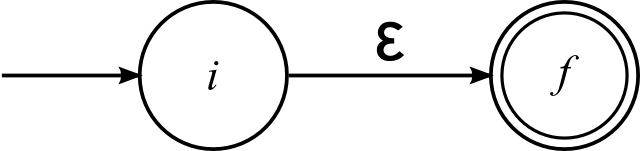
\includegraphics[width=0.40\textwidth]{pics/epsilon.png}  
    \end{center}
\end{frame}

\begin{frame}
  \transwipe[direction=90]
  \frametitle{Построение КА по РВ: символ}
    \begin{center}
      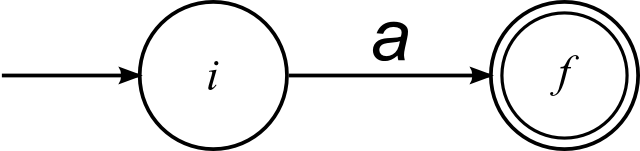
\includegraphics[width=0.40\textwidth]{pics/terminal.png}  
    \end{center}
\end{frame}

\begin{frame}
  \transwipe[direction=90]
  \frametitle{Построение КА по РВ: объединение $p \mid q$}
    \begin{center}
      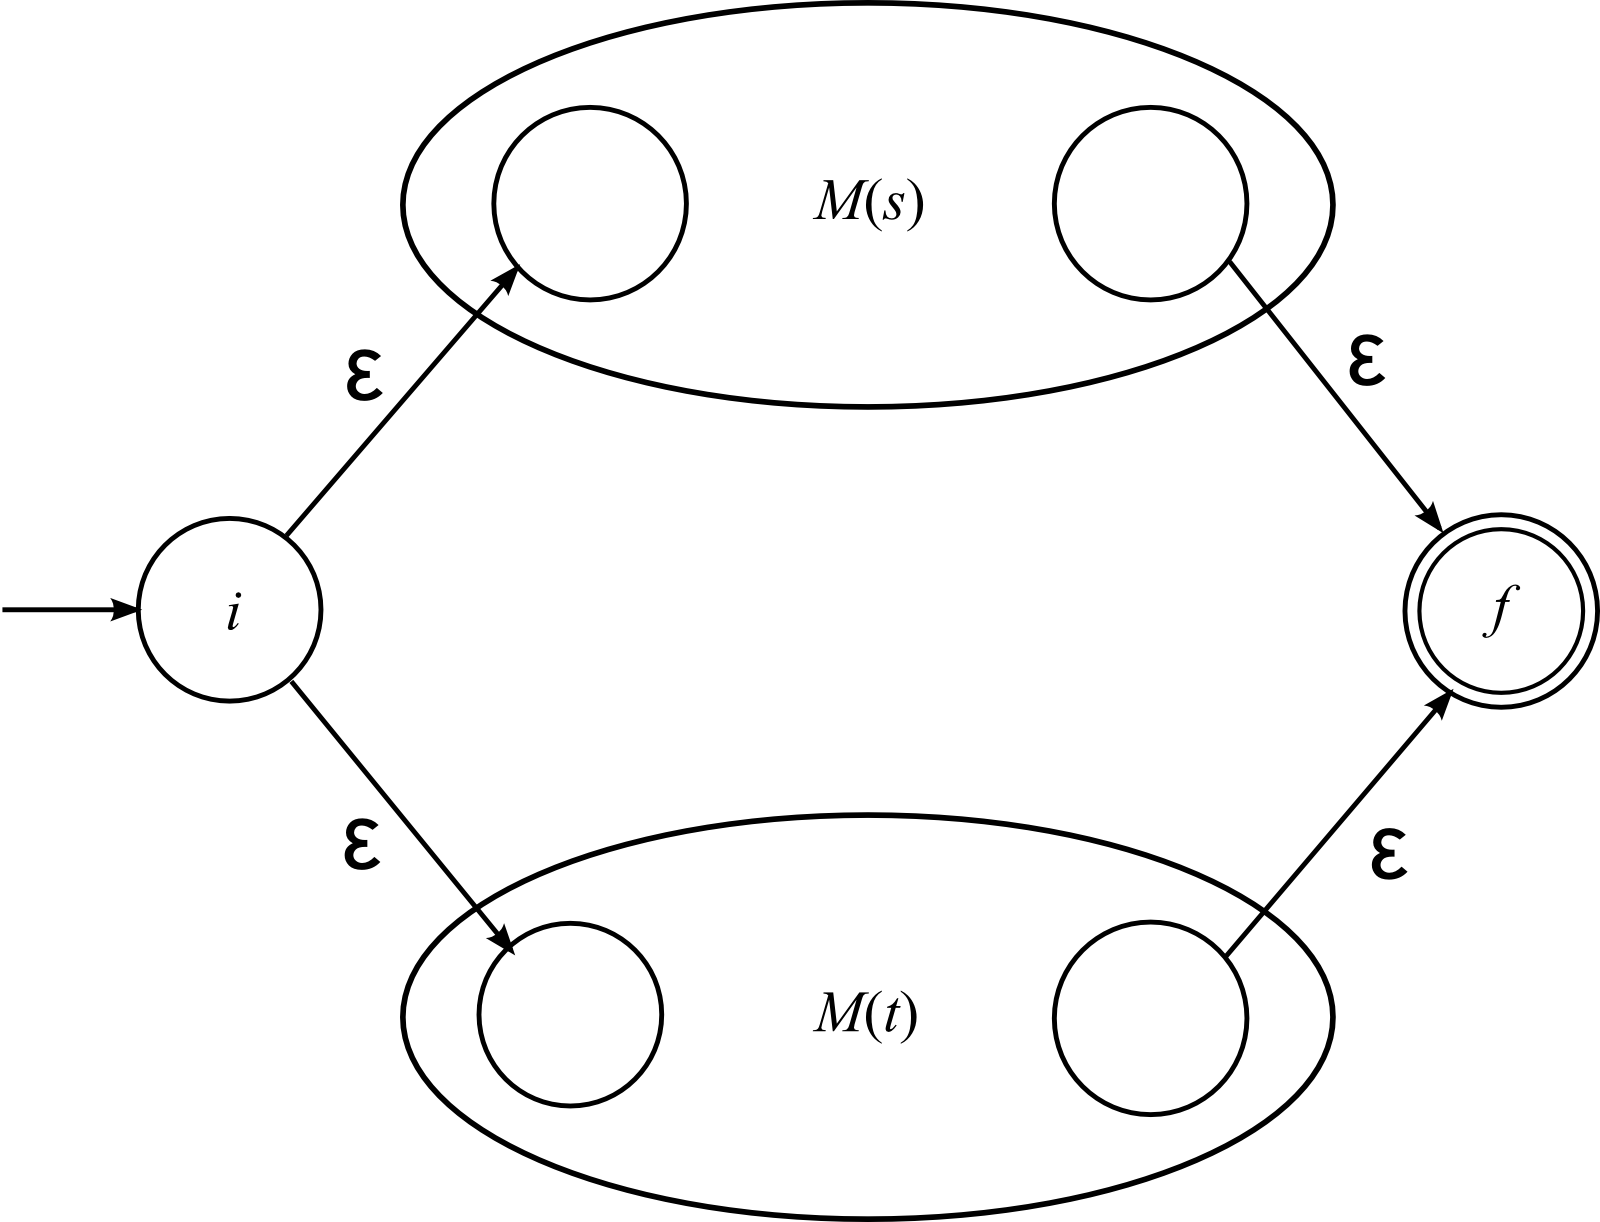
\includegraphics[width=0.80\textwidth]{pics/union.png}  
    \end{center}
\end{frame}

\begin{frame}
  \transwipe[direction=90]
  \frametitle{Построение КА по РВ: конкатенация $p q$}
    \begin{center}
      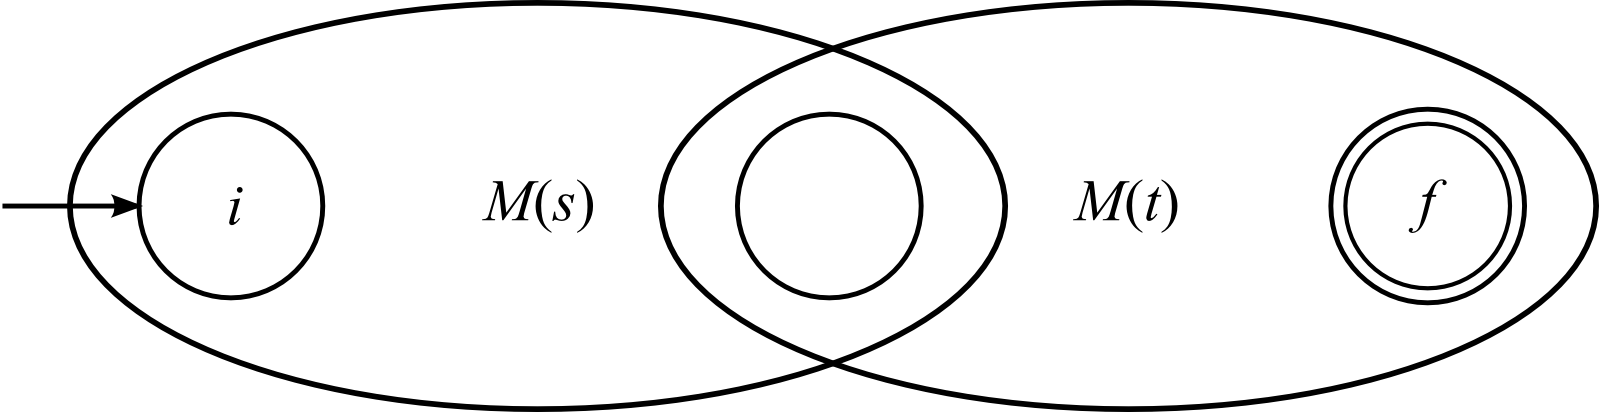
\includegraphics[width=0.80\textwidth]{pics/concat.png}  
    \end{center}
\end{frame}

\begin{frame}
  \transwipe[direction=90]
  \frametitle{Построение КА по РВ: итерация $p^*$}
    \begin{center}
      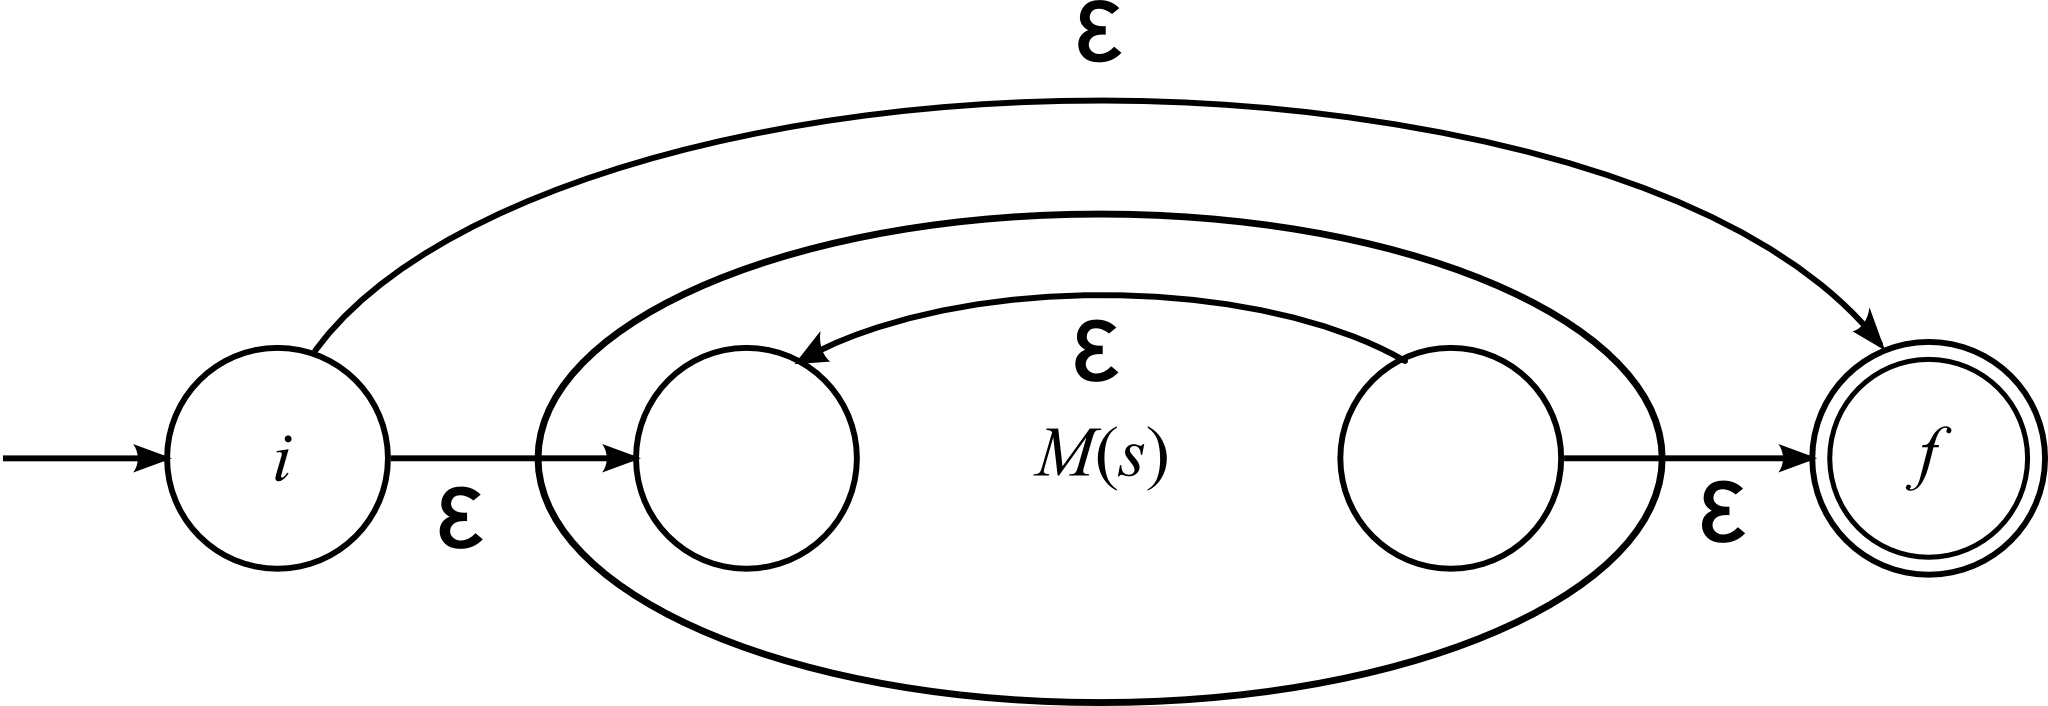
\includegraphics[width=0.80\textwidth]{pics/star.png}  
    \end{center}
\end{frame}

\begin{frame}
  \transwipe[direction=90]
  \frametitle{Теорема Клини: доказательство $\Rightarrow$}
  
  \begin{rutheorem}
   Классы автоматных и регулярных языков \emph{эквивалентны}
  \end{rutheorem}
  
  \begin{proof} 
   $\Rightarrow: $
    Построим регулярное выражение по конечному автомату методом исключения состояний
    
    Идея: на ребрах пишем регулярные выражения, соответсвующие путям между вершинами, последовательно исключаем состояния   
    
  \end{proof}
\end{frame}

\begin{frame}
  \transwipe[direction=90]
  \frametitle{Исключение состояния $s$}

  \begin{myauto}
    \node[state] (s)                    {s};
    \node[state] (p) [above left of=s]  {p};
    \node[state] (q) [above right of=s] {q};

    \path[->] (p) edge [bend left=15] node [above] {$R_3$} (q)
                  edge                node [below] {$R_1$} (s)
              (s) edge                node [below] {$R_2$} (q)
                  edge [loop above]   node [above] {$R$}   ()
              ;
  \end{myauto}

  \begin{myauto}
    \node[state] (s)                    {s};
    \node[state] (p) [above left of=s]  {p};
    \node[state] (q) [above right of=s] {q};

    \path[->] (p) edge [bend left=15] node [above] {$R_3 \mid R_1 R^* R_2$} (q)
                  edge                node [below] {$R_1$}                  (s)
              (s) edge                node [below] {$R_2$}                  (q)
                  edge [loop above]   node [above] {$R$}                    ()
              ;
  \end{myauto}
\end{frame}

\begin{frame}
  \transwipe[direction=90]
  \frametitle{Исключение состояния $s$: удаление ребер и вершины}
  \begin{myauto}[2.2]
    \node[state] (s)                    {s};
    \node[state] (p) [above left of=s]  {p};
    \node[state] (q) [above right of=s] {q};

    \path[->] (p) edge [bend left=15] node [above] {$R_3 \mid R_1 R^* R_2$} (q)
              ;
  \end{myauto}
  
  \vfill

  \begin{myauto}
    \node[state] (p)              {p};
    \node[state] (q) [right of=p] {q};

    \path[->] (p) edge [bend left=15] node [above] {$R_3 \mid R_1 R^* R_2$} (q)
              ;
  \end{myauto}
\end{frame}

\begin{frame}
  \transwipe[direction=90]
  \frametitle{Исключение состояний: последний шаг}
  \begin{myauto}
    \node[state,initial]   (p)              {p};
    \node[state,accepting] (q) [right of=p] {q};

    \path[->] (p) edge [bend left=15] node [above] {$S$} (q)
                  edge [loop above]   node [above] {$R$} ()
              (q) edge [loop above]   node [above] {$U$} ()
                  edge [bend left=15] node [below] {$T$} (p)
              ;
  \end{myauto}
  
  \vfill

    \[ (R^* \mid S U^* T)^* S U^* \]
\end{frame}

\begin{frame}
  \transwipe[direction=90]
  \frametitle{Исключение состояний: последний шаг}
  \begin{myauto}
    \node[state,initial,accepting] (q) {q};

    \path[->] (q) edge [loop above] node [above] {$R$} ()
              ;
  \end{myauto}
    
  \vfill 

    \[ R^* \]
\end{frame}

\begin{frame}
  \transwipe[direction=90]
  \frametitle{Исключение состояний: пример}

  \begin{myauto}[2]
    \node[state,initial]   (q_01)                      {A};
    \node[state]           (q_2)  [right=of q_01]      {B};
    \node[state,accepting] (q_3)  [right=of q_2]       {C};
    \node[state]           (q_4)  [above right=of q_3] {D};
    \node[state]           (q_56) [right=of q_3] {E};

    \path[->] (q_01) edge [loop above]    node [above] {$1$}   ()
                     edge [bend left=15]  node [above] {$0$}   (q_2)
              (q_2)  edge                 node [below] {$1$}   (q_3)
                     edge [bend left=15]  node [below] {$0$}   (q_01)
              (q_3)  edge [bend left=15]  node [above] {$1$}   (q_56)
                     edge                 node [above] {$0$}   (q_4)
              (q_4)  edge [loop right]    node [right] {$0,1$} ()
              (q_56) edge [bend left=15]  node [below] {$1$}   (q_3)
                     edge                 node [right] {$0$}   (q_4);
  \end{myauto} 

  \begin{myauto}[2]
    \node[state,initial]   (q_01)                 {A};
    \node[state]           (q_2)  [right=of q_01] {B};
    \node[state,accepting] (q_3)  [right=of q_2]  {C};

    \path[->] (q_01) edge [loop above]    node [above] {$1$}      ()
                     edge [bend left=15]  node [above] {$0$}      (q_2)
              (q_2)  edge                 node [below] {$1$}      (q_3)
                     edge [bend left=15]  node [below] {$0$}      (q_01)
              (q_3)  edge [loop right]    node [right] {$(11)^*$} ()
              ;
  \end{myauto} 

  \begin{myauto}[3.5]
    \node[state,initial]   (q_01)                  {A};
    \node[state,accepting] (q_3)  [right=of q_01]  {C};

    \path[->] (q_01) edge              node [above] {$1^*0(\varepsilon \mid 01^*0)^*1$} (q_3)
              (q_3)  edge [loop right] node [right] {$(11)^*$}      ()
              ;
  \end{myauto} 

  \[ 1^*0(\varepsilon \mid 01^*0)^*1 (11)^* \]
\end{frame}

\begin{frame}
  \transwipe[direction=90]
  \frametitle{Свойства регулярных выражений}
  \begin{itemize}
    \item $a \mid a = a$
    \item $a \mid \varnothing = a$
    \item $a \mid b = b \mid a$
    \item $a \mid (b \mid c) = (a \mid b) \mid c$
    \item $a(bc) = (ab)c$
    \item $\{\varepsilon \} a = a \{ \varepsilon \} = a $
    \item $\varnothing a = a \varnothing = \varnothing$
    \item $a (b\mid c) = ab \mid ac$
    \item $(a \mid b) c = ac \mid bc $
    \item $\{\varepsilon \} \mid aa^* \subseteq a^*$
    \item $\{\varepsilon \} \mid a^*a \subseteq a^*$
    \item $ab \subseteq b \Rightarrow a^* b \subseteq b$
    \item $ab \subseteq a \Rightarrow a b^* \subseteq a$
        
  \end{itemize}
\end{frame}



\begin{frame}[fragile]
  \transwipe[direction=90]
  \frametitle{Регулярная грамматика}
  \textbf{Праволинейная грамматика} --- грамматика, все правила которой имеют следующий вид:
  \begin{itemize}
    \item $A \to a B, A \to a \text{ или } A \to \varepsilon \text{, где } A, B \in V_N, a \in V_T$
  \end{itemize}


  \textbf{Леволинейная грамматика} --- грамматика, все правила которой имеют следующий вид:
  \begin{itemize}
    \item $A \to B a, A \to a \text{ или } A \to \varepsilon \text{, где } A, B \in V_N, a \in V_T$
  \end{itemize}

\pause 

  \begin{rutheorem}[]
    Пусть L --- формальный язык. 

    $\exists G_r$ --- праволинейная грамматика, т.ч. $L = L(G_r) \Leftrightarrow$ 
    
    $\exists G_l$ --- леволинейная грамматика, т.ч. $L = L(G_l) $
  \end{rutheorem}
\pause
  \textbf{Регулярная грамматика} --- праволинейная или леволинейная грамматика
\end{frame}



\begin{frame}[fragile]
  \transwipe[direction=90]
  \frametitle{Эквивалентность регулярной грамматики и НКА}
  Алгоритм построения НКА $\langle Q, \Sigma, q_0, \delta, F \rangle$ по праволинейной грамматике $\langle V_T, V_N, P, S \rangle$
  
  \begin{itemize}
    \item $Q = V_N \cup \{q_f\}$
    \item $\forall (A \to a B) \in P: \delta (A, a) = B$
    \item $\forall (A \to a) \in P: \delta (A, a) = q_f$
    \item $q_0 = S$
    \item $\forall (B \to \varepsilon) \in P: B \in F$
  \end{itemize}
\end{frame}


\begin{frame}[fragile]
  \transwipe[direction=90]
  \frametitle{Пример построения НКА по регулярной грамматике}
  \begin{align*}
    S &\to a A \mid a S \mid \varepsilon \\ 
    A &\to b A \mid b \\ 
  \end{align*}
  
  \begin{myauto}
    \node[state,initial,accepting] (q_0)                {S};
    \node[state]                   (q_1) [right of=q_0] {A}; 
    \node[state,accepting]         (q_2) [right of=q_1] {$q_f$}; 

    \path[->] (q_0) edge [loop above]   node [above] {$a$} ()
                    edge                node [above] {$a$} (q_1)
              (q_1) edge [loop above]   node [above] {$b$} () 
                    edge                node [above] {$b$} (q_2)
              ;
  \end{myauto}
\end{frame}

\begin{frame}[fragile]
  \transwipe[direction=90]
  \frametitle{Эквивалентность регулярной грамматики и НКА}
  Алгоритм построения праволинейной грамматики $\langle V_T, V_N, P, S \rangle$ по НКА $\langle Q, \Sigma, q_0, \delta, F \rangle$

  \begin{itemize}
    \item $V_N = Q$
    \item $V_T = \Sigma$
    \item $\forall \delta(A, a) = B : (A \to a B) \in P$
    \item $\forall B \in F: (B \to \varepsilon) \in P$
    \item $S = q_0$
    \item Опционально: удалить $\varepsilon$-правила и бесполезные символы
  \end{itemize}
\end{frame}

\begin{frame}[fragile]
  \transwipe[direction=90]
  \frametitle{Пример построения регулярной грамматики по НКА}
  \begin{myauto}
    \node[state,initial,accepting] (q_0)                {S};
    \node[state]                   (q_1) [right of=q_0] {B}; 
    \node[state,accepting]         (q_2) [right of=q_1] {F}; 

    \path[->] (q_0) edge [loop above]   node [above] {$a$} ()
                    edge                node [above] {$a$} (q_1)
              (q_1) edge [loop above]   node [above] {$b$} () 
                    edge                node [above] {$a$} (q_2)
              ;
  \end{myauto}

  \vfill 
  
  \begin{align*}
    S &\to a B \mid a S \\ 
    B &\to b B \mid a F \\ 
    F &\to \varepsilon  
  \end{align*}
\end{frame}

\begin{frame}[fragile]
  \transwipe[direction=90]
  \frametitle{Пример построения регулярной грамматики по НКА}
  \begin{myauto}
    \node[state,initial,accepting] (q_0)                {S};
    \node[state]                   (q_1) [right of=q_0] {B}; 
    \node[state,accepting]         (q_2) [right of=q_1] {F}; 

    \path[->] (q_0) edge [loop above]   node [above] {$a$} ()
                    edge                node [above] {$a$} (q_1)
              (q_1) edge [loop above]   node [above] {$b$} () 
                    edge                node [above] {$a$} (q_2)
              ;
  \end{myauto}

  \vfill 
  
  \begin{align*}
    S &\to a B \mid a S \\ 
    B &\to b B \mid a 
  \end{align*}
\end{frame}

\begin{frame}[fragile]
  \transwipe[direction=90]
  \frametitle{Лемма о разрастании (о накачке)}
  \begin{rutheorem}
  $L$ --- регулярный язык над $\Sigma \Rightarrow \exists n: \forall \omega \in L, | \omega | > n$
  
    $\exists x, y, z \in \Sigma^*: \, xyz = \omega, y \neq \varepsilon, |xy| \leq n,$
    
     $ \forall k \geq 0: \, x y^k z \in L$
  \end{rutheorem}
  
  \begin{proof}
  Строим автомат, распознающий $L$.
  
  Обозначаем за $n$ число состояний автомата.
  
  Слово длины большей, чем $n$, обязано при разборе пройти через одно состояние дважды --- получили цикл. 

  Метка цикла --- искомое $y$, по циклу можно пройти сколько угодно раз.
  
  \end{proof}

\end{frame}


\begin{frame}[fragile]
  \transwipe[direction=90]
  \frametitle{Использование леммы о накачке}

  \[ L = \{ (^k )^k \mid k \geq 0\} \]

  \begin{itemize}
    \item Предполагаем, что $L$ --- регулярный язык, значит выполняется лемма о накачке
    \item Берем $n$ из леммы, рассматриваем слово $(^n )^n$ 
    \item Его можно разбить на $xyz, y \neq \varepsilon, |xy| \leq n$
    \item $|xy| \leq n \Rightarrow y = (^b, b > 0$
    \item Берем $k = 2: xy^kz = (^{n+b} )^n$, что не принадлежит $L$
    \item Получили противоречие $\Rightarrow L$  не регулярен
  \end{itemize}
  
\end{frame}

\begin{frame}[fragile]
  \transwipe[direction=90]
  \frametitle{Использование леммы о накачке}
\[ L = \{ a^{k^2} \mid k \geq 0\} \]

  \begin{itemize}
    \item Предполагаем, что $L$ --- регулярный язык, значит выполняется лемма о накачке 
    \item Берем $n$ из леммы, рассматриваем слово $a^{(n+1)^2}$ 
    \begin{itemize}
      \item Слово $a^{n^2}$ не подойдет, потому что $|a^{n^2}| = n, \text{ где } n = 1$
    \end{itemize}
    \item Его можно разбить на $xyz, y \neq \varepsilon, |xy| \leq n$
    \item Берем $k = 0: xy^0z = xz$
    \item $n^2 < n^2 + n + 1 = (n+1)^2 - n \leq |xz| \leq (n+1)^2 - 1 < (n+1)^2$
    \item Длина слова $xz$ находится между двумя соседними полными квадратами, поэтому это слово не в $L$
    \item Получили противоречие $\Rightarrow L$  не регулярен
  \end{itemize}
  
\end{frame}

\begin{frame}[fragile]
  \transwipe[direction=90]
  \frametitle{Резюме}
  \begin{itemize}
    \item ДКА, НКА, НКА с $\varepsilon$-переходами, регулярные выражения, регулярные грамматики --- все эти формализмы задают один класс (регулярных) языков и эквивалентны друг другу
    \item Проверка принадлежности слова регулярному языку осуществляется за $O(n)$ и не требует дополнительной памяти
    \item Класс регулярных языков обладает хорошими свойствами, прост и нагляден
    \item С помощью леммы о накачке можно доказать нерегулярность языка
  \end{itemize}
  
\end{frame}


\end{document}
